\begin{figure}
  \centering
  \subfigure[SFI]{
    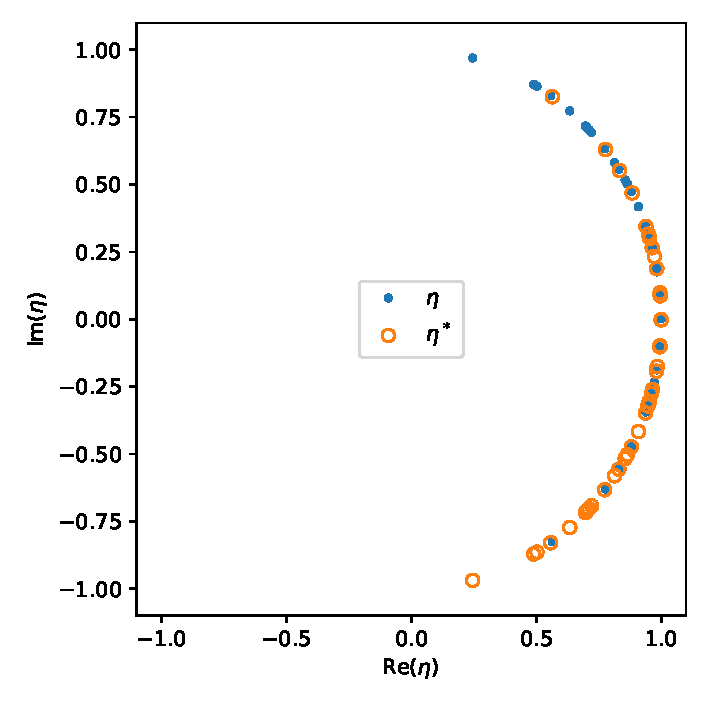
\includegraphics[width=0.44\textwidth]{../Plots/qmbs_sfim_N=06_tduration=0.5_Vrr=100_Omega=1.pdf}
  }
  \subfigure[PXP]{
    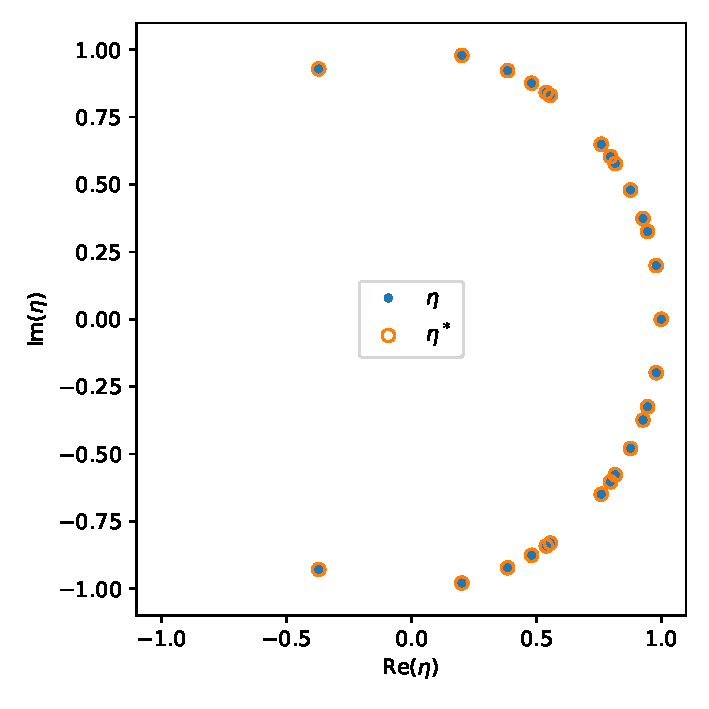
\includegraphics[width=0.44\textwidth]{../Plots/qmbs_pxp_N=06_tduration=0.5_Omega=1.pdf}
  }
  \caption{Eigenvalues, $\eta$ and their complex conjugates, $\eta^*$,
    of the the propagator, plotted in the complex place for $N=6$,
    $\Omega t=0.5$, for (a) SFI with $V_{rr}=100\Omega$ and (b) PXP
    Hamiltonians}
\end{figure}

\begin{figure}
  \centering
  \subfigure[SFI]{
    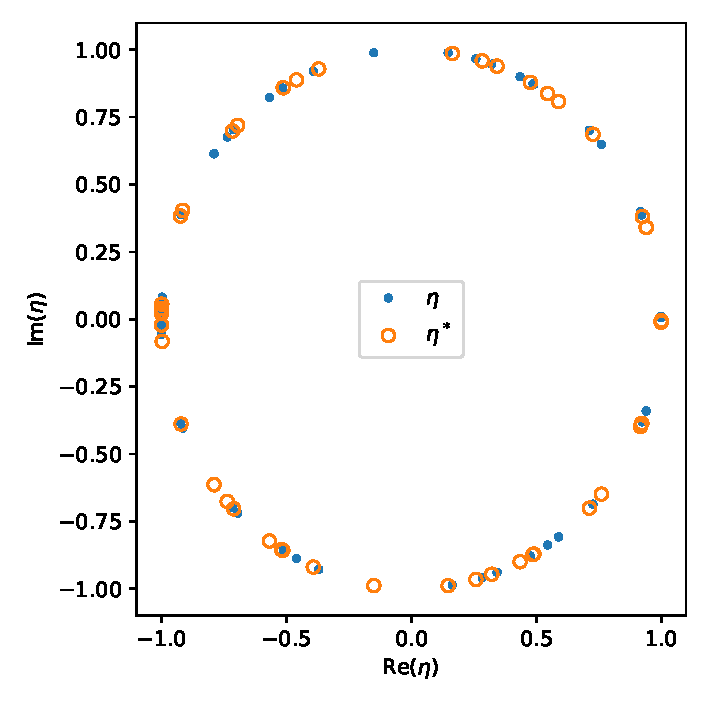
\includegraphics[width=0.44\textwidth]{../Plots/qmbs_sfim_N=06_tduration=2_Vrr=100_Omega=1.pdf}
  }
  \subfigure[PXP]{
    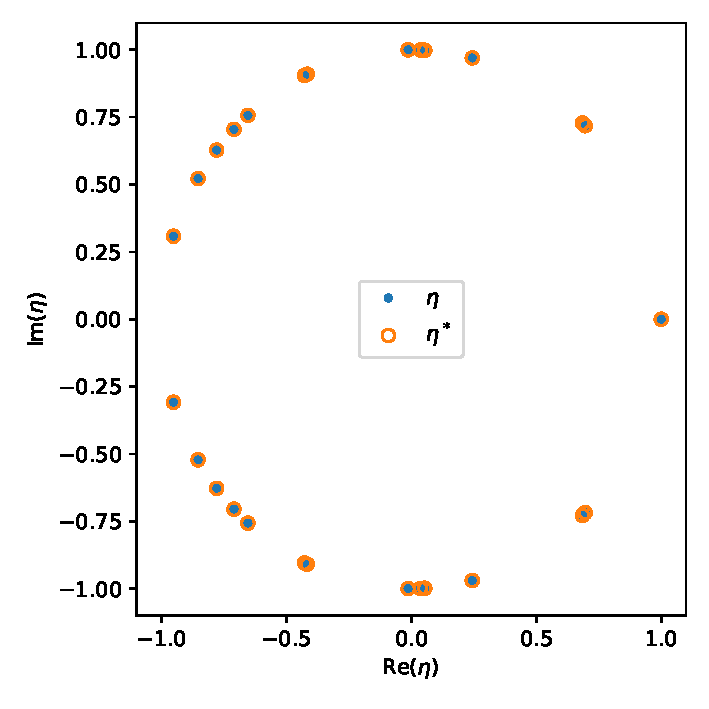
\includegraphics[width=0.44\textwidth]{../Plots/qmbs_pxp_N=06_tduration=2_Omega=1.pdf}
  }
  \caption{Eigenvalues, $\eta$ and their complex conjugates, $\eta^*$,
    of the the propagator, plotted in the complex place for $N=6$,
    $\Omega t=2$, for (a) SFI with $V_{rr}=100\Omega$ and (b) PXP
    Hamiltonians}
\end{figure}


\begin{figure}
  \centering
  \subfigure[SFI]{
    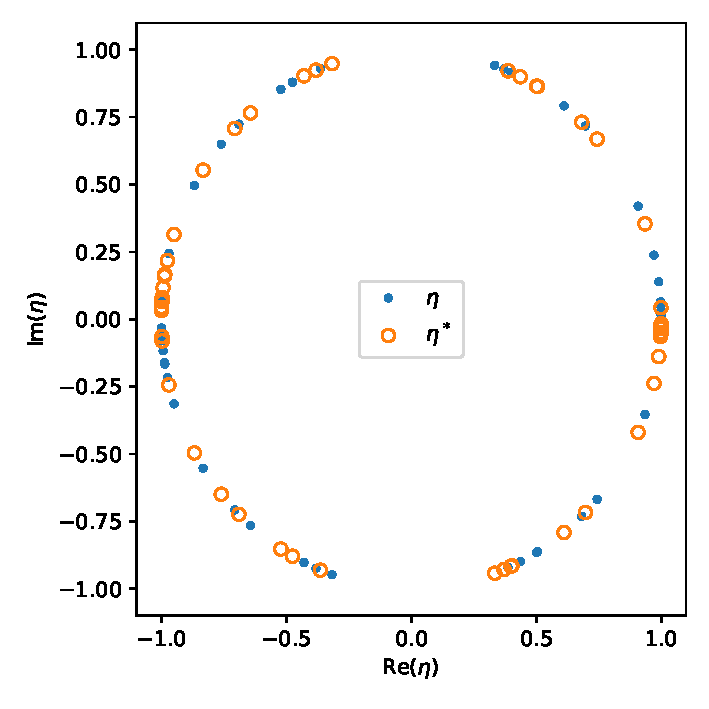
\includegraphics[width=0.44\textwidth]{../Plots/qmbs_sfim_N=06_tduration=6_Vrr=100_Omega=1.pdf}
  }
  \subfigure[PXP]{
    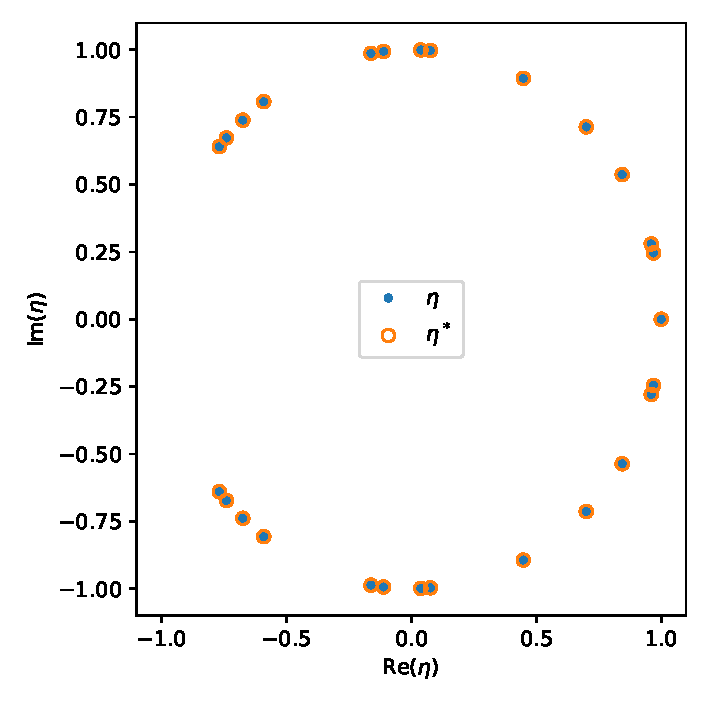
\includegraphics[width=0.44\textwidth]{../Plots/qmbs_pxp_N=06_tduration=6_Omega=1.pdf}
  }
  \caption{Eigenvalues, $\eta$ and their complex conjugates, $\eta^*$,
    of the the propagator, plotted in the complex place for $N=6$,
    $\Omega t=6$, for (a) SFI with $V_{rr}=100\Omega$ and (b) PXP
    Hamiltonians}
\end{figure}


\begin{figure}
  \centering
  \subfigure[SFI]{
    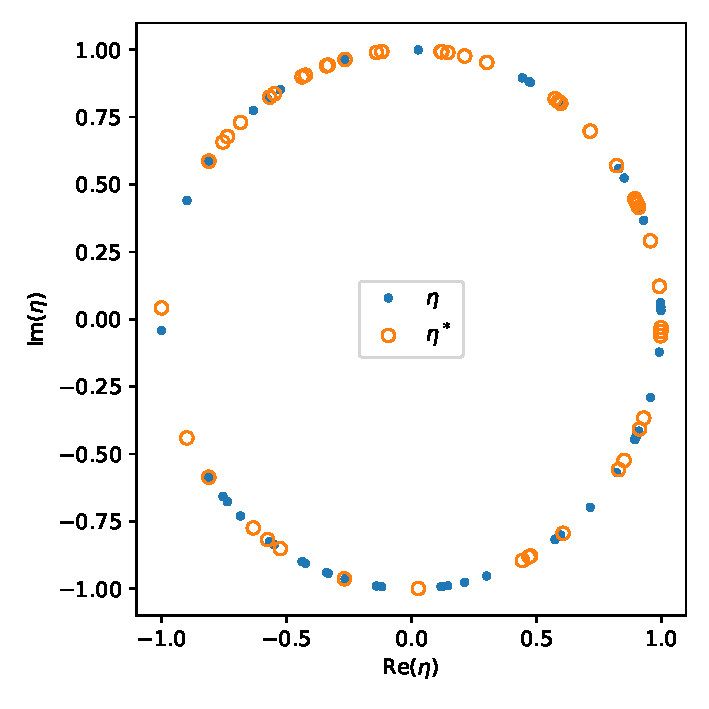
\includegraphics[width=0.44\textwidth]{../Plots/qmbs_sfim_N=06_tduration=11_Vrr=100_Omega=1.pdf}
  }
  \subfigure[PXP]{
    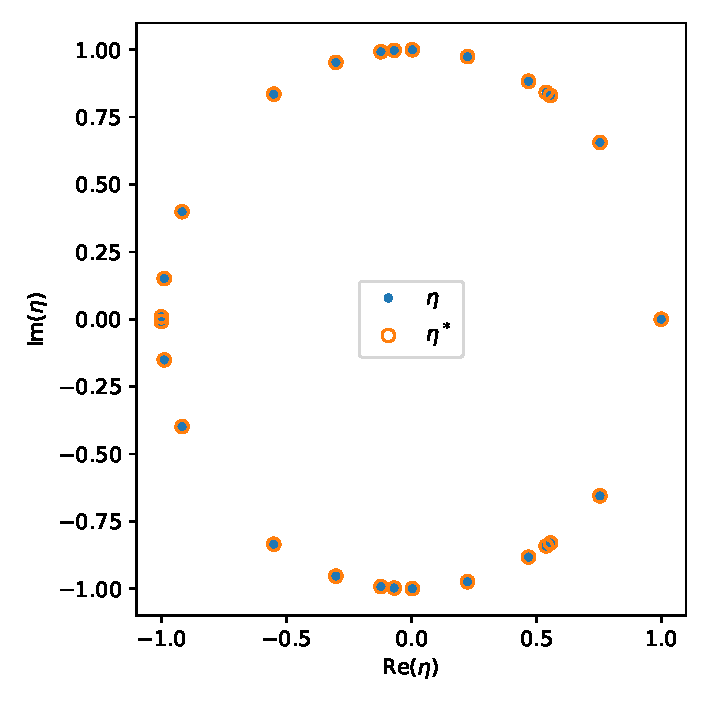
\includegraphics[width=0.44\textwidth]{../Plots/qmbs_pxp_N=06_tduration=11_Omega=1.pdf}
  }
  \caption{Eigenvalues, $\eta$ and their complex conjugates, $\eta^*$,
    of the the propagator, plotted in the complex place for $N=6$,
    $\Omega t=11$, for (a) SFI with $V_{rr}=100\Omega$ and (b) PXP
    Hamiltonians}
\end{figure}

%%%%%%%%%%%%%%%%

\begin{figure}
  \centering
  \subfigure[SFI]{
    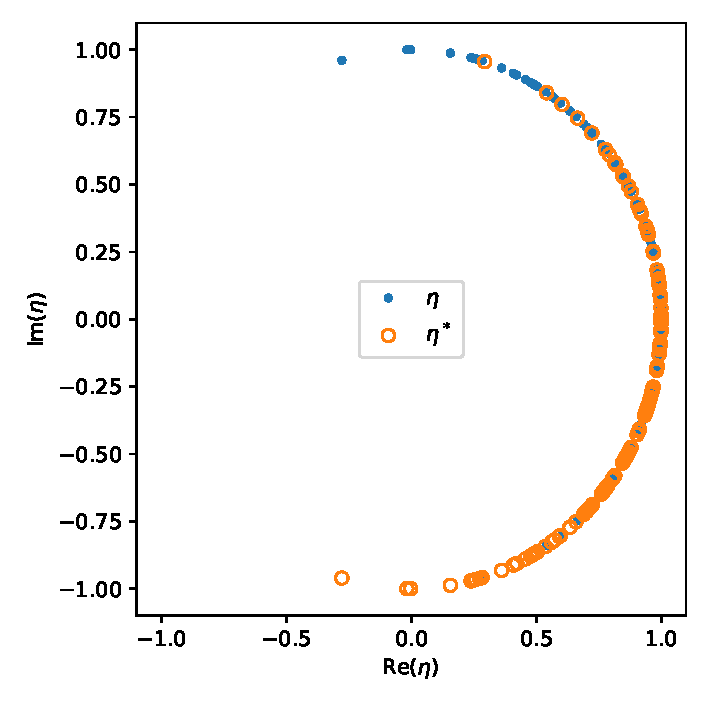
\includegraphics[width=0.44\textwidth]{../Plots/qmbs_sfim_N=08_tduration=0.5_Vrr=100_Omega=1.pdf}
  }
  \subfigure[PXP]{
    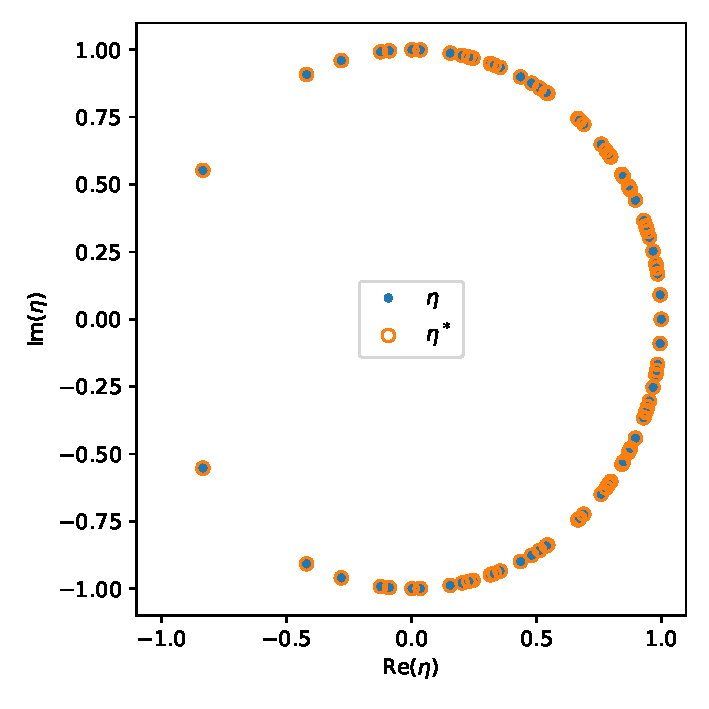
\includegraphics[width=0.44\textwidth]{../Plots/qmbs_pxp_N=08_tduration=0.5_Omega=1.pdf}
  }
  \caption{Eigenvalues, $\eta$ and their complex conjugates, $\eta^*$,
    of the the propagator, plotted in the complex place for $N=8$,
    $\Omega t=0.5$, for (a) SFI with $V_{rr}=100\Omega$ and (b) PXP
    Hamiltonians}
\end{figure}

\begin{figure}
  \centering
  \subfigure[SFI]{
    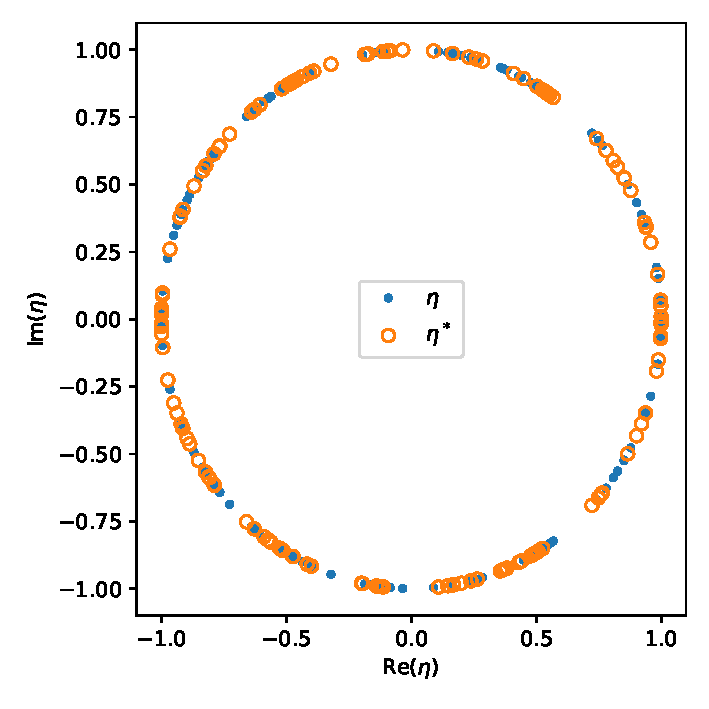
\includegraphics[width=0.44\textwidth]{../Plots/qmbs_sfim_N=08_tduration=2_Vrr=100_Omega=1.pdf}
  }
  \subfigure[PXP]{
    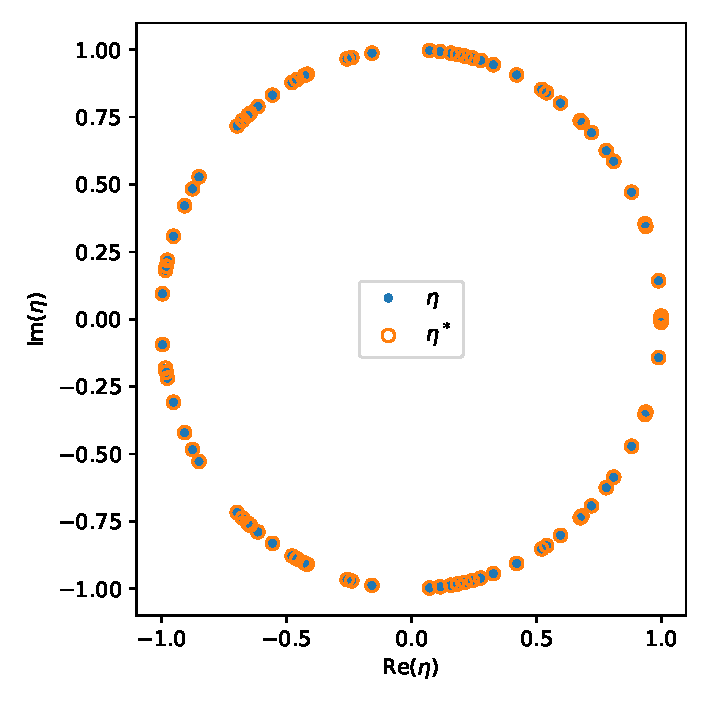
\includegraphics[width=0.44\textwidth]{../Plots/qmbs_pxp_N=08_tduration=2_Omega=1.pdf}
  }
  \caption{Eigenvalues, $\eta$ and their complex conjugates, $\eta^*$,
    of the the propagator, plotted in the complex place for $N=8$,
    $\Omega t=2$, for (a) SFI with $V_{rr}=100\Omega$ and (b) PXP
    Hamiltonians}
\end{figure}


\begin{figure}
  \centering
  \subfigure[SFI]{
    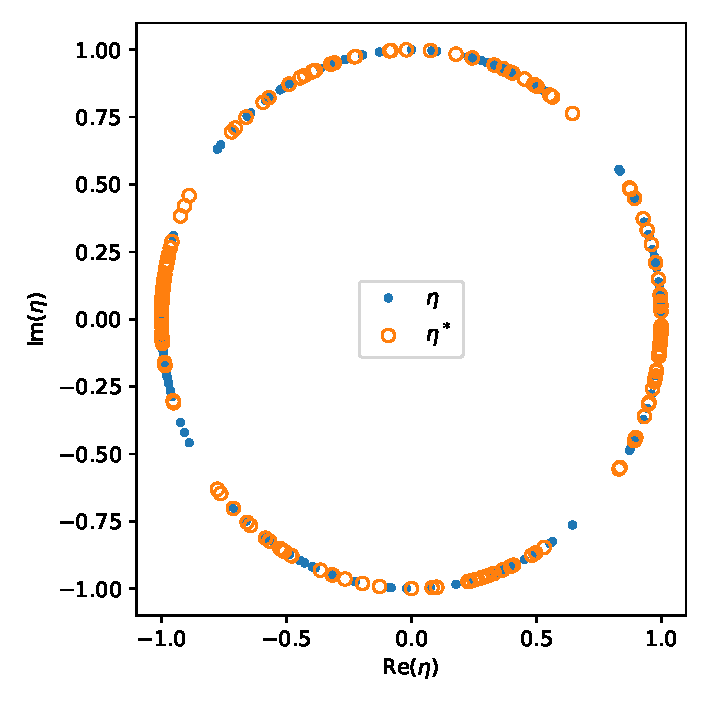
\includegraphics[width=0.44\textwidth]{../Plots/qmbs_sfim_N=08_tduration=6_Vrr=100_Omega=1.pdf}
  }
  \subfigure[PXP]{
    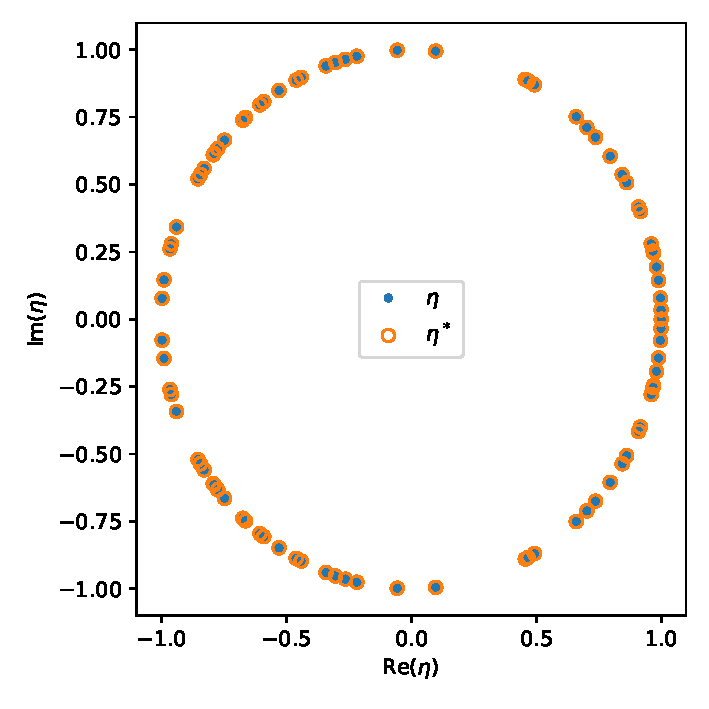
\includegraphics[width=0.44\textwidth]{../Plots/qmbs_pxp_N=08_tduration=6_Omega=1.pdf}
  }
  \caption{Eigenvalues, $\eta$ and their complex conjugates, $\eta^*$,
    of the the propagator, plotted in the complex place for $N=8$,
    $\Omega t=6$, for (a) SFI with $V_{rr}=100\Omega$ and (b) PXP
    Hamiltonians}
\end{figure}


\begin{figure}
  \centering
  \subfigure[SFI]{
    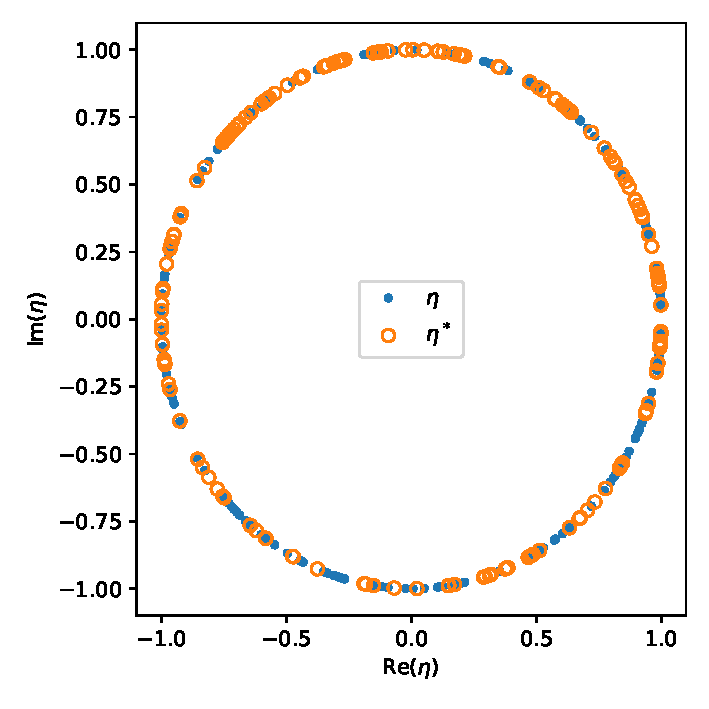
\includegraphics[width=0.44\textwidth]{../Plots/qmbs_sfim_N=08_tduration=11_Vrr=100_Omega=1.pdf}
  }
  \subfigure[PXP]{
    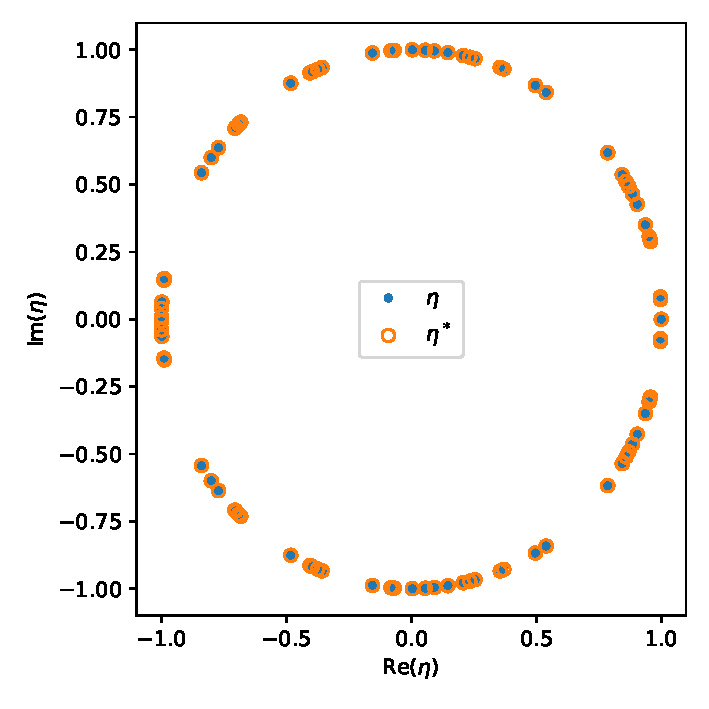
\includegraphics[width=0.44\textwidth]{../Plots/qmbs_pxp_N=08_tduration=11_Omega=1.pdf}
  }
  \caption{Eigenvalues, $\eta$ and their complex conjugates, $\eta^*$,
    of the the propagator, plotted in the complex place for $N=8$,
    $\Omega t=11$, for (a) SFI with $V_{rr}=100\Omega$ and (b) PXP
    Hamiltonians}
\end{figure}

%%%%%%%%%%%%%%%

\begin{figure}
  \centering
  \subfigure[SFI]{
    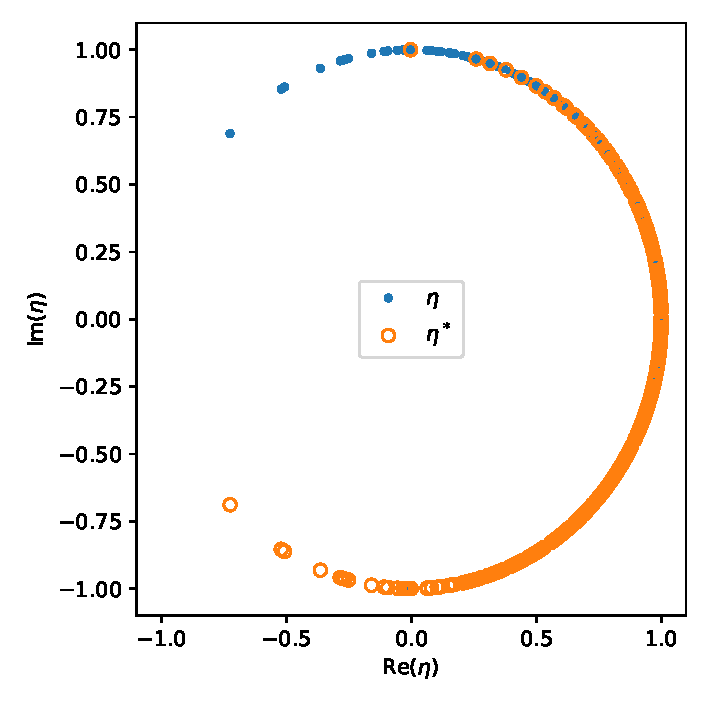
\includegraphics[width=0.44\textwidth]{../Plots/qmbs_sfim_N=10_tduration=0.5_Vrr=100_Omega=1.pdf}
  }
  \subfigure[PXP]{
    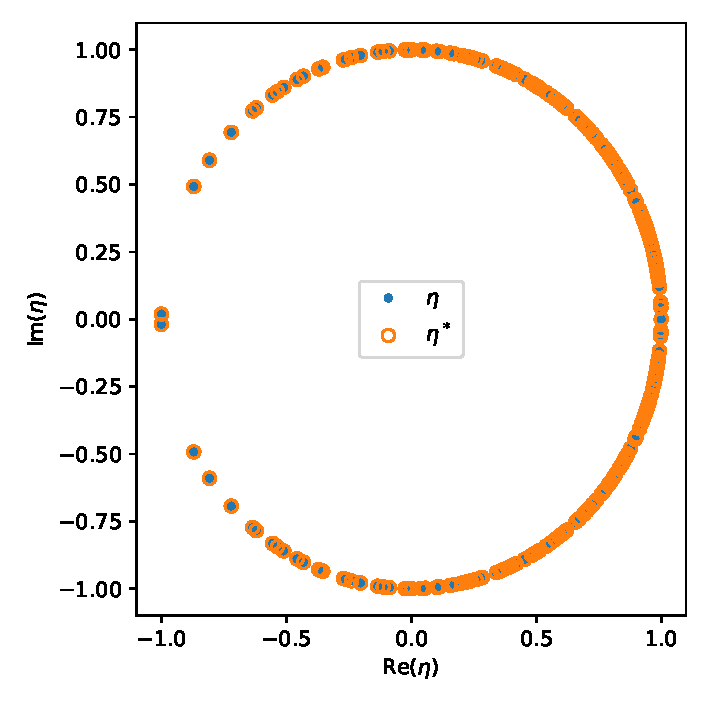
\includegraphics[width=0.44\textwidth]{../Plots/qmbs_pxp_N=10_tduration=0.5_Omega=1.pdf}
  }
  \caption{Eigenvalues, $\eta$ and their complex conjugates, $\eta^*$,
    of the the propagator, plotted in the complex place for $N=10$,
    $\Omega t=0.5$, for (a) SFI with $V_{rr}=100\Omega$ and (b) PXP
    Hamiltonians}
\end{figure}

\begin{figure}
  \centering
  \subfigure[SFI]{
    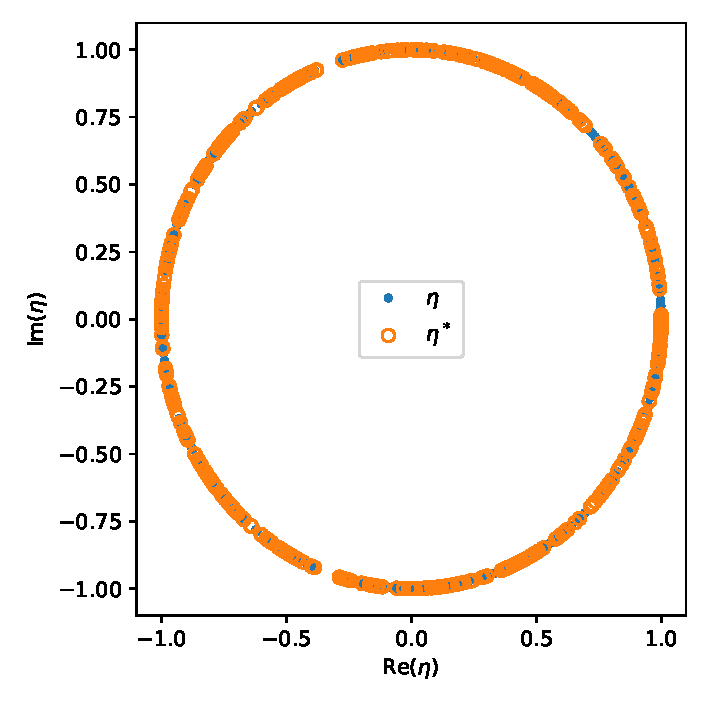
\includegraphics[width=0.44\textwidth]{../Plots/qmbs_sfim_N=10_tduration=2_Vrr=100_Omega=1.pdf}
  }
  \subfigure[PXP]{
    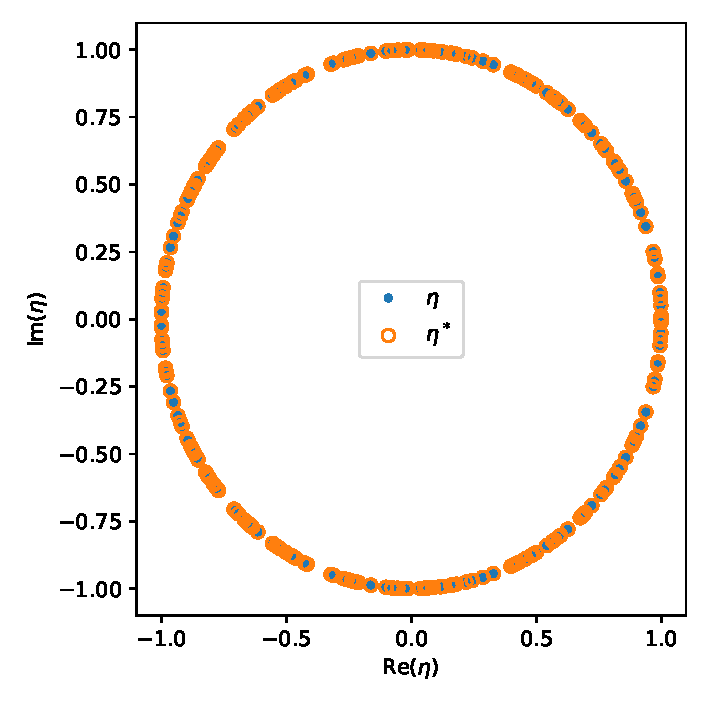
\includegraphics[width=0.44\textwidth]{../Plots/qmbs_pxp_N=10_tduration=2_Omega=1.pdf}
  }
  \caption{Eigenvalues, $\eta$ and their complex conjugates, $\eta^*$,
    of the the propagator, plotted in the complex place for $N=10$,
    $\Omega t=2$, for (a) SFI with $V_{rr}=100\Omega$ and (b) PXP
    Hamiltonians}
\end{figure}


\begin{figure}
  \centering
  \subfigure[SFI]{
    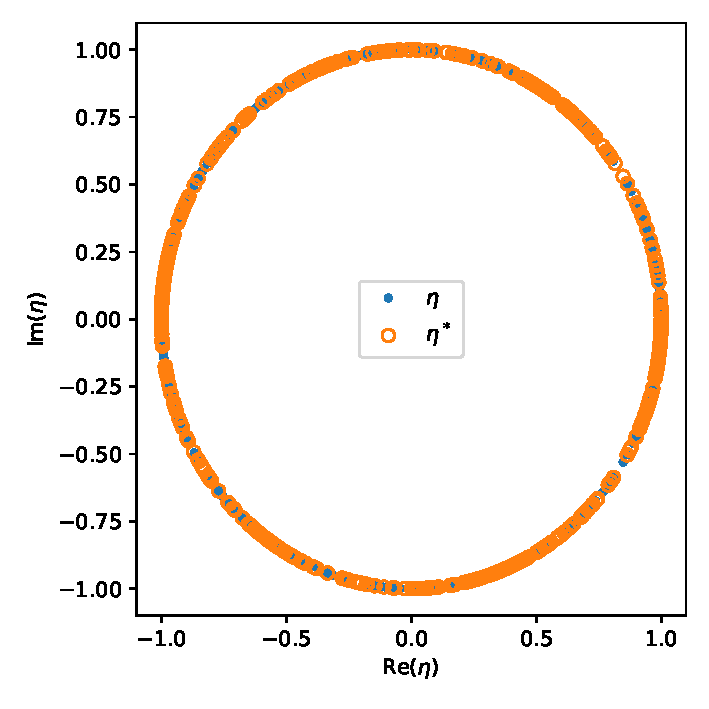
\includegraphics[width=0.44\textwidth]{../Plots/qmbs_sfim_N=10_tduration=6_Vrr=100_Omega=1.pdf}
  }
  \subfigure[PXP]{
    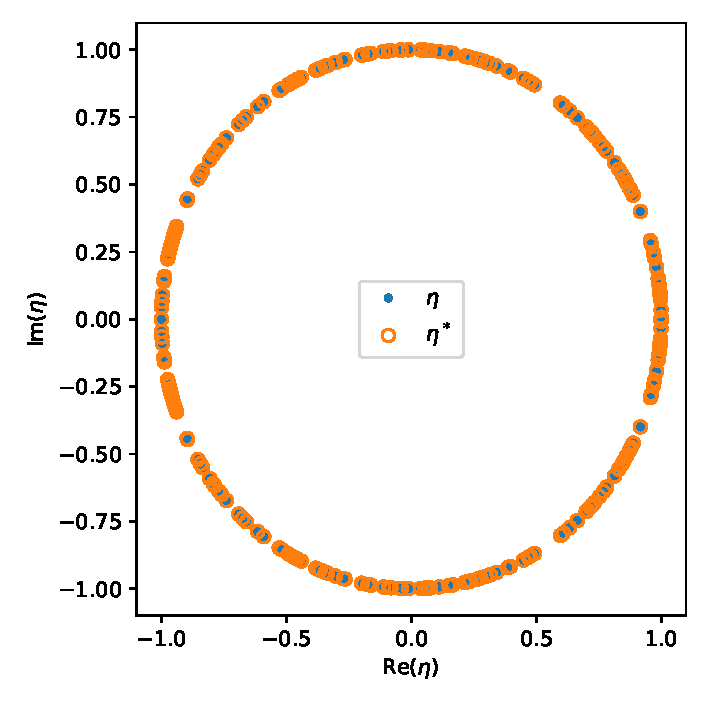
\includegraphics[width=0.44\textwidth]{../Plots/qmbs_pxp_N=10_tduration=6_Omega=1.pdf}
  }
  \caption{Eigenvalues, $\eta$ and their complex conjugates, $\eta^*$,
    of the the propagator, plotted in the complex place for $N=10$,
    $\Omega t=6$, for (a) SFI with $V_{rr}=100\Omega$ and (b) PXP
    Hamiltonians}
\end{figure}


\begin{figure}
  \centering
  \subfigure[SFI]{
    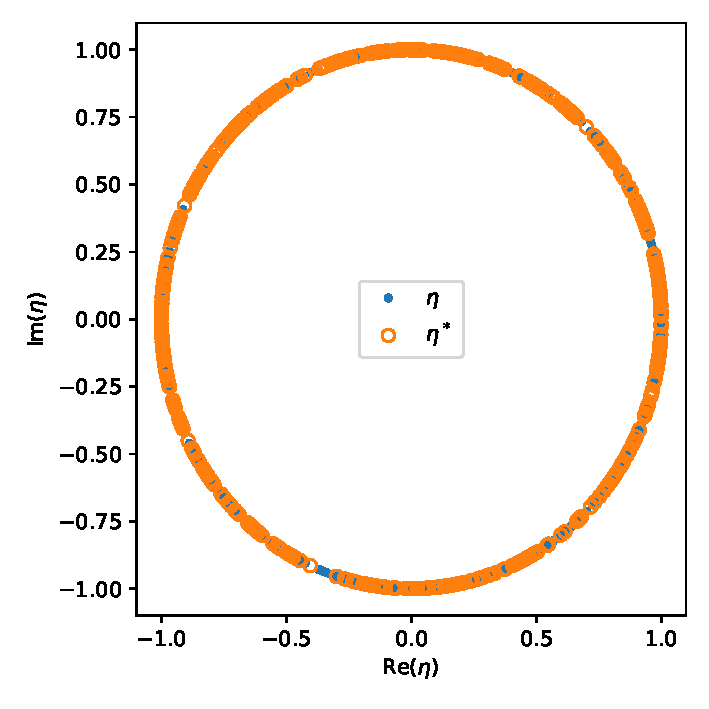
\includegraphics[width=0.44\textwidth]{../Plots/qmbs_sfim_N=10_tduration=11_Vrr=100_Omega=1.pdf}
  }
  \subfigure[PXP]{
    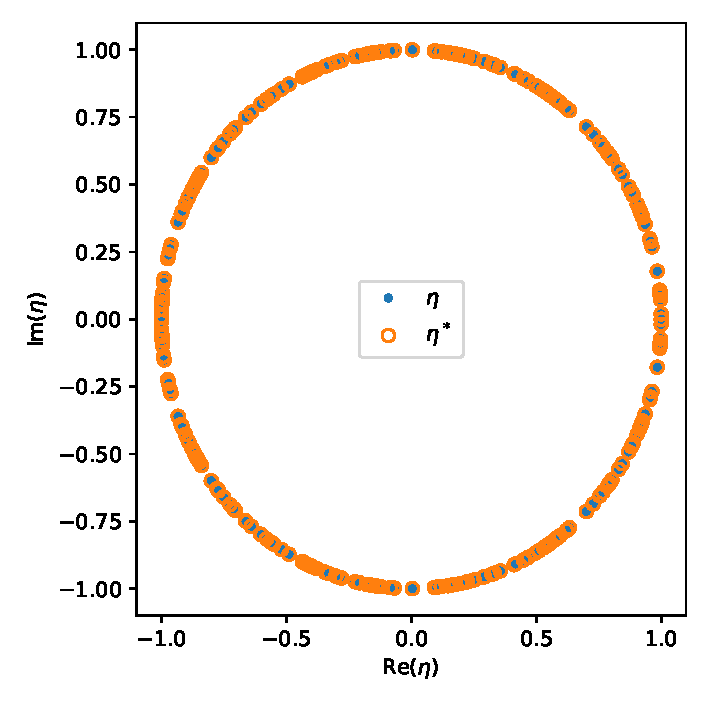
\includegraphics[width=0.44\textwidth]{../Plots/qmbs_pxp_N=10_tduration=11_Omega=1.pdf}
  }
  \caption{Eigenvalues, $\eta$ and their complex conjugates, $\eta^*$,
    of the the propagator, plotted in the complex place for $N=10$
    $\Omega t=11$, for (a) SFI with $V_{rr}=100\Omega$ and (b) PXP
    Hamiltonians}
\end{figure}
